\chapter{Sprints}
\settocdepth{chapter}
\label{Sprints}

\section{Sprint 0}
The design draft was drawn as a paper prototype (see section \ref{ss:paper_prototype}), and the group performed a demonstration to the customer. He was satisfied with the idea, and it created a great discussion about how the group should continue working.

The group are satisfied with their own efforts. Heaps of work are accomplished, and everyone are motivated to keep working next sprint.
    
The group agreed that they should be more effective during their work sessions, aiming on accomplishing more. To achieve this it is important that everyone takes responsibility of keeping the group on track, and  make sure everyone are concentrated on the tasks at hand.

\begin{figure}[ht]
\centering
    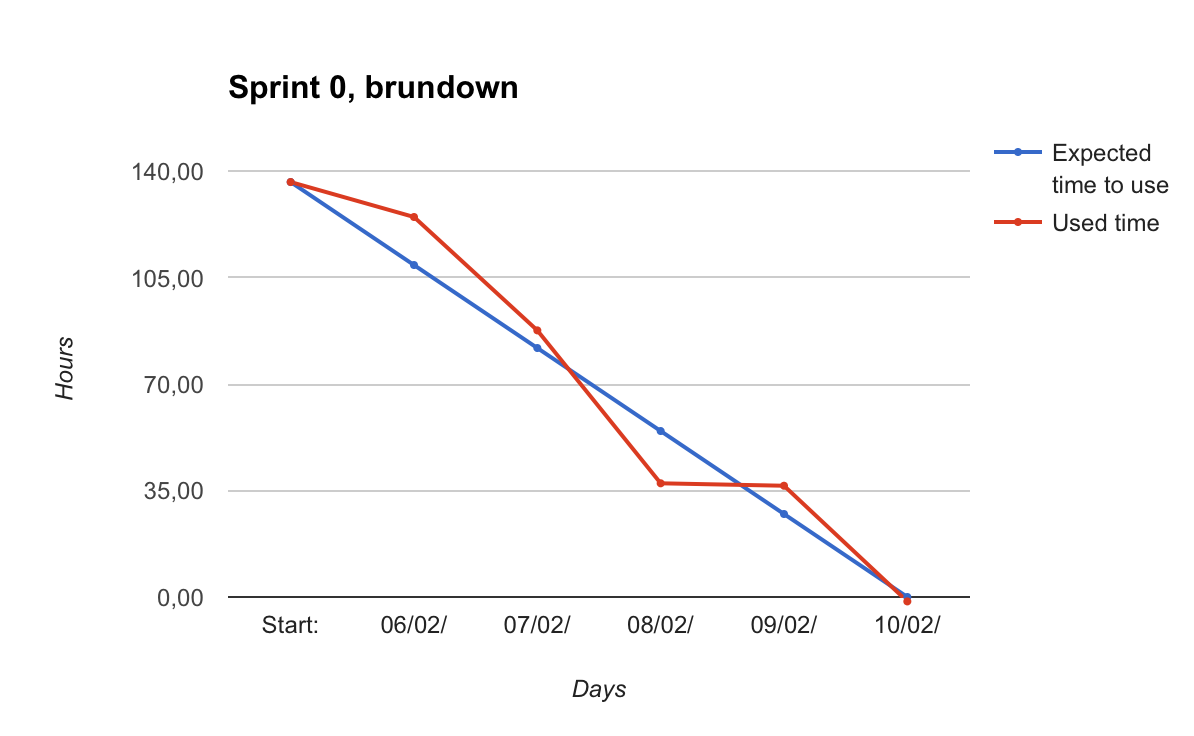
\includegraphics[width=0.8\textwidth]{fig/sprint0}
\caption{Sprint 0, burndown}
\end{figure}

\begin{figure}[ht]
\centering
    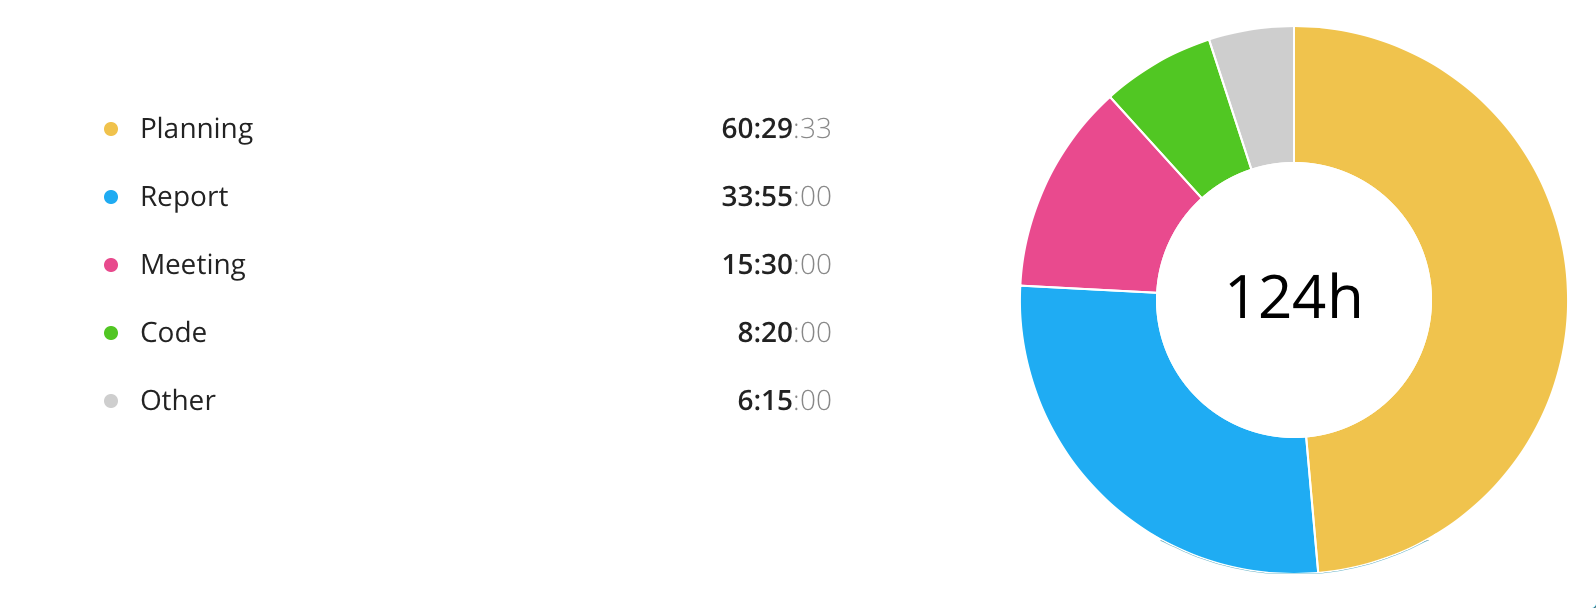
\includegraphics[width=0.8\textwidth]{fig/sprint0-diagram}
\caption{Sprint 0, hours distributed to work tasks}
\end{figure}

\section{Sprint 1}
\label{Sprints-sprint1}
The group concluded this was very inconvenient this early on in the development process, and all resources were necessary to complete the sprint goal. To manage such problems in the future, the group updated their risk analysis (see section \ref{updated_risk_analysis}). 

Because of the misunderstanding with the customer, the group had a discussion on how much time to actually spend on the project. After resolving the misunderstanding with customer, the group concluded that the already scheduled hours should remain.

\begin{figure}[ht]
\centering
    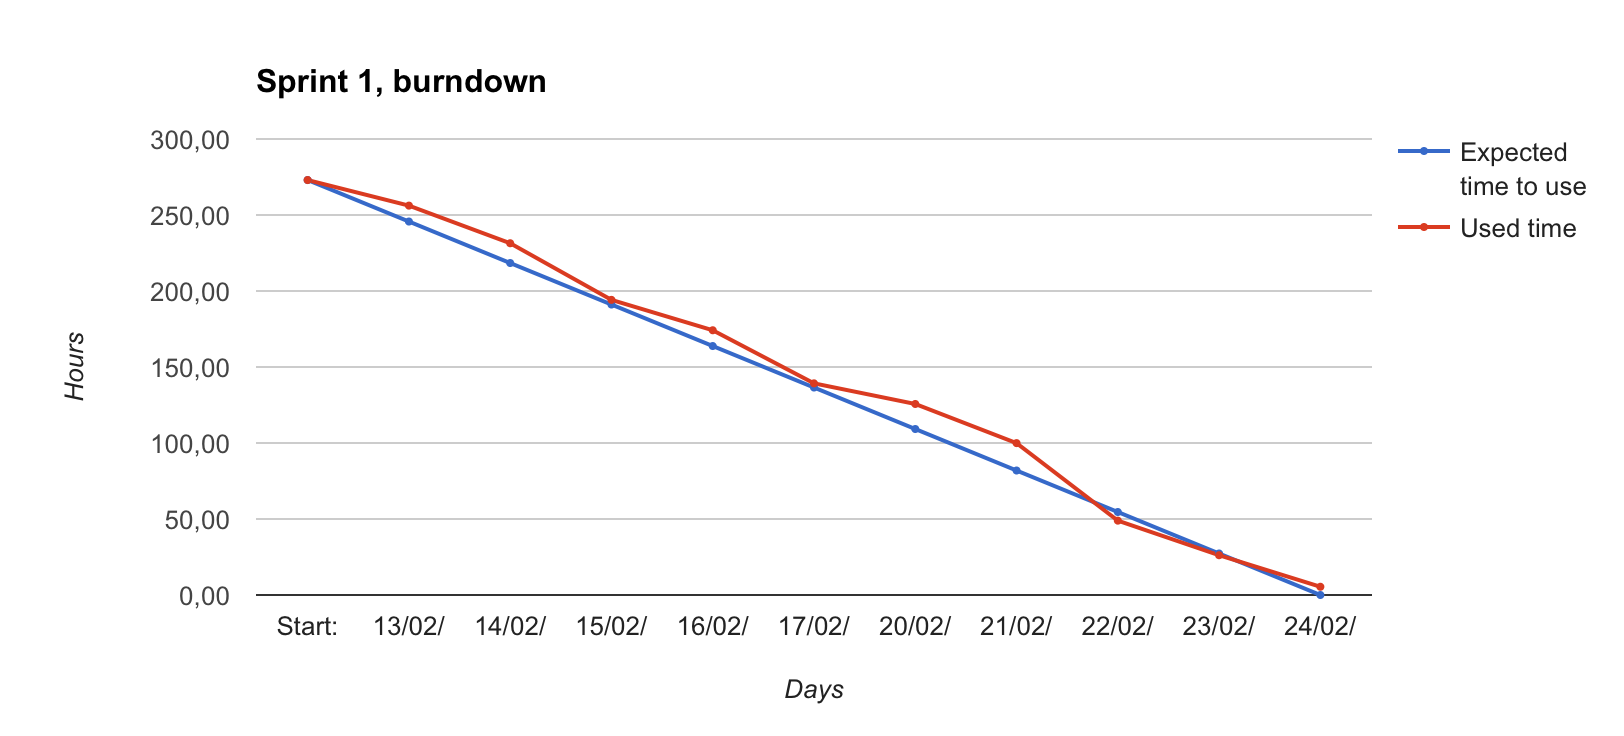
\includegraphics[width=0.8\textwidth]{fig/sprint1}
\caption{Sprint 1, burndown}
\end{figure}

\begin{figure}[ht]
\centering
    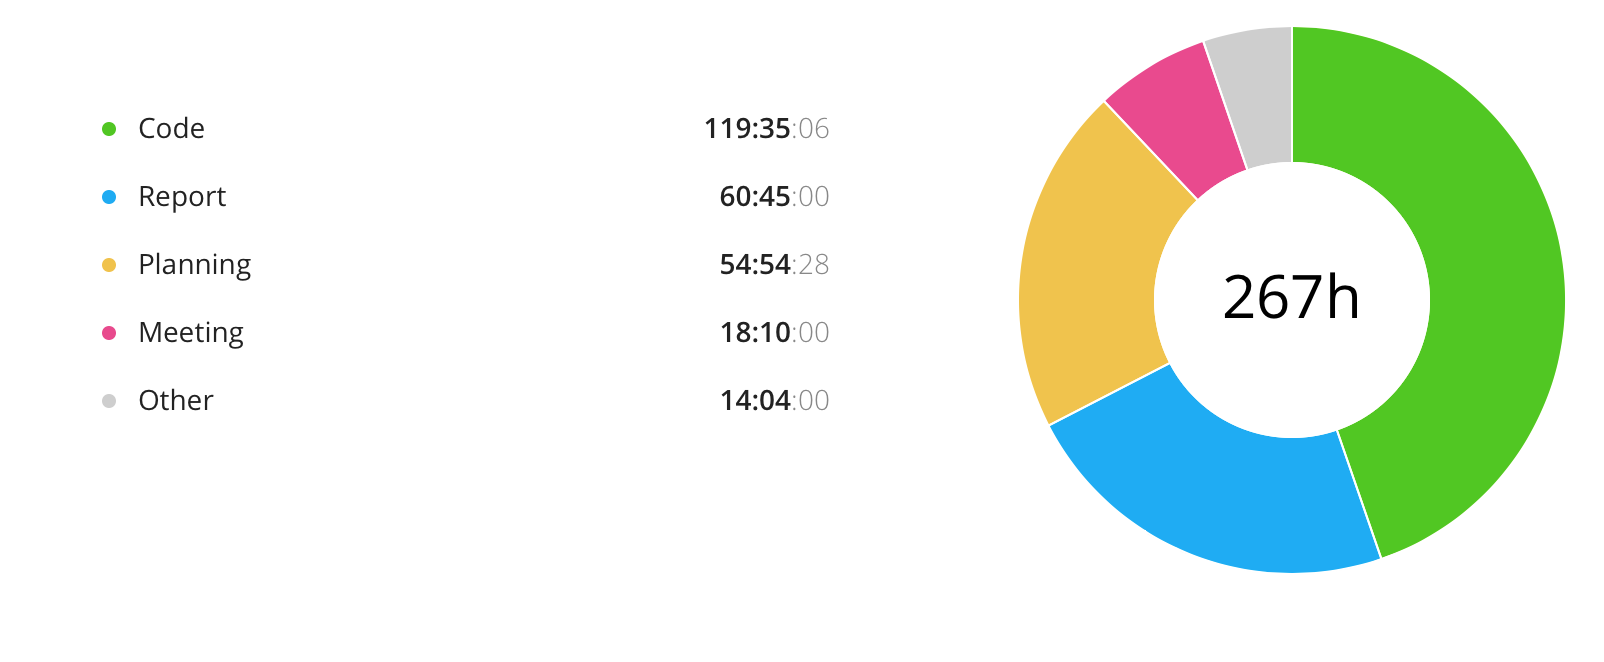
\includegraphics[width=0.8\textwidth]{fig/sprint1-diagram}
\caption{Sprint 1, hours distributed to work tasks}
\end{figure}

\section{Sprint 2}
\label{Sprints-sprint2}
The group experienced couple of problems during this sprint. Firstly, the group came across problems trying to implement the possibility to filter the activities. Initially the group had chosen to use flux, to manage the data flow in the application \cite{flux}. With further research and attempts trying to implement the flux pattern, the group realized it would not be sufficient in this project, as the application was required to support asynchronous actions. Midway in the sprint the group decided to use Redux (see \ref{redux}). To solve this issue the group was required to complete further research on how this should be implemented, this consumed more of the sprint than first expected.

During sprint 1 a set of milestones were defined and arranged after priority, which the group used to define the sprint backlogs. Midway in sprint 2 the customer arouse the desire for one of the final milestones, \textit{"first version of release up and running on server"}, to be completed. To fulfill the customer's desire the group highly prioritized this milestone, which induced difficulties completing the original issues in the sprint backlog. To encounter this issue the group decided to re-prioritize the backlog subsequently after the request from the customer. Moving the milestone at hand to sprint 2 and relocate the milestone "Sign up for activity" to sprint 3. 

Even tough the group encountered a couple of problems, the group was happy with what they had managed to accomplish. These problems affected what was included in the sprint backlog, and subsequently the sprint goal. Still a lot of functionality was implemented and the group worked very well during this period. As an improvement to the upcoming sprints the group decided to become better at focusing on the issues in the sprint backlog.

\begin{figure}[ht]
\centering
    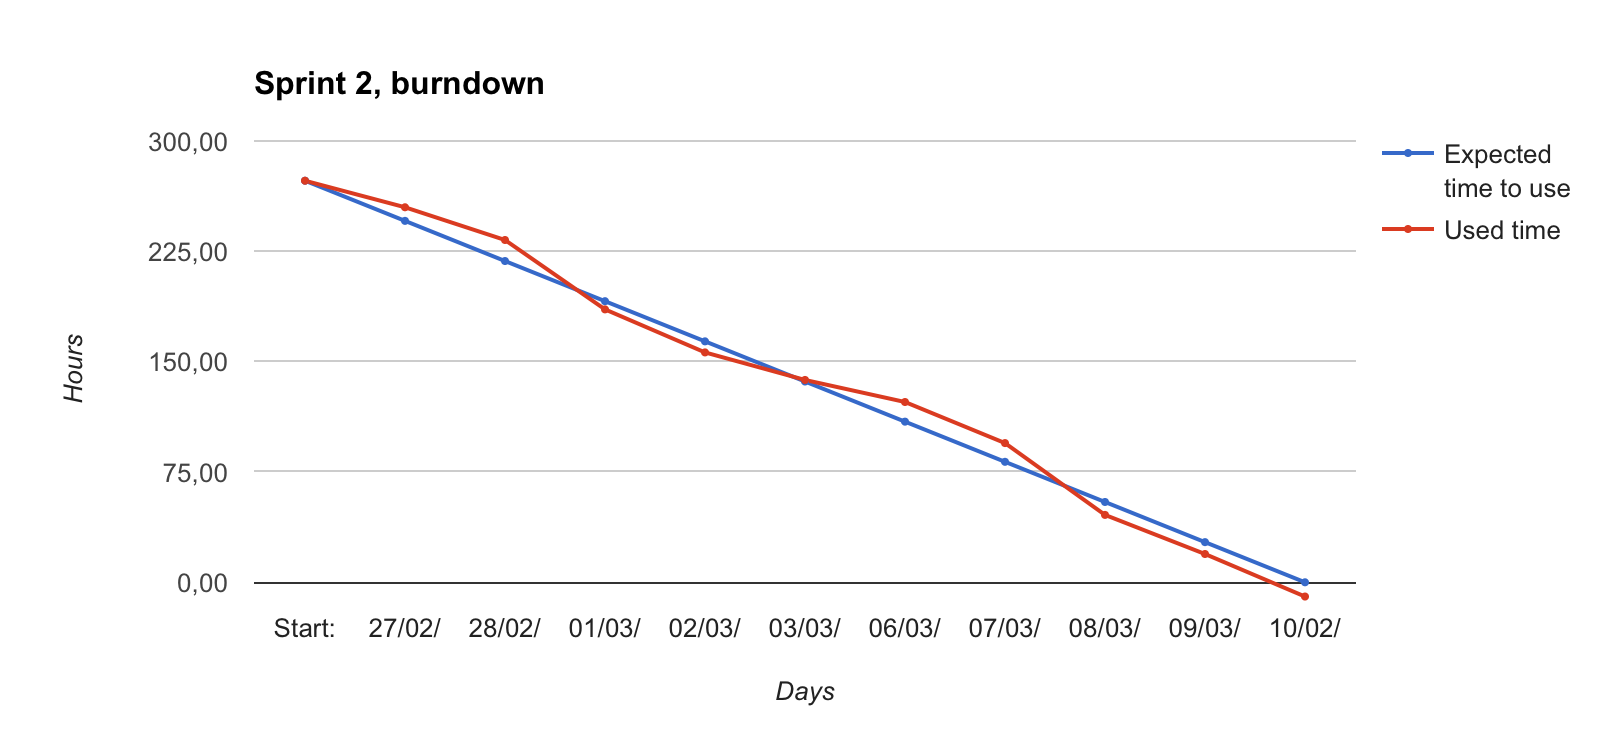
\includegraphics[width=0.8\textwidth]{fig/sprint2}
\caption{Sprint 2, burndown}
\end{figure}

\begin{figure}[ht]
\centering
    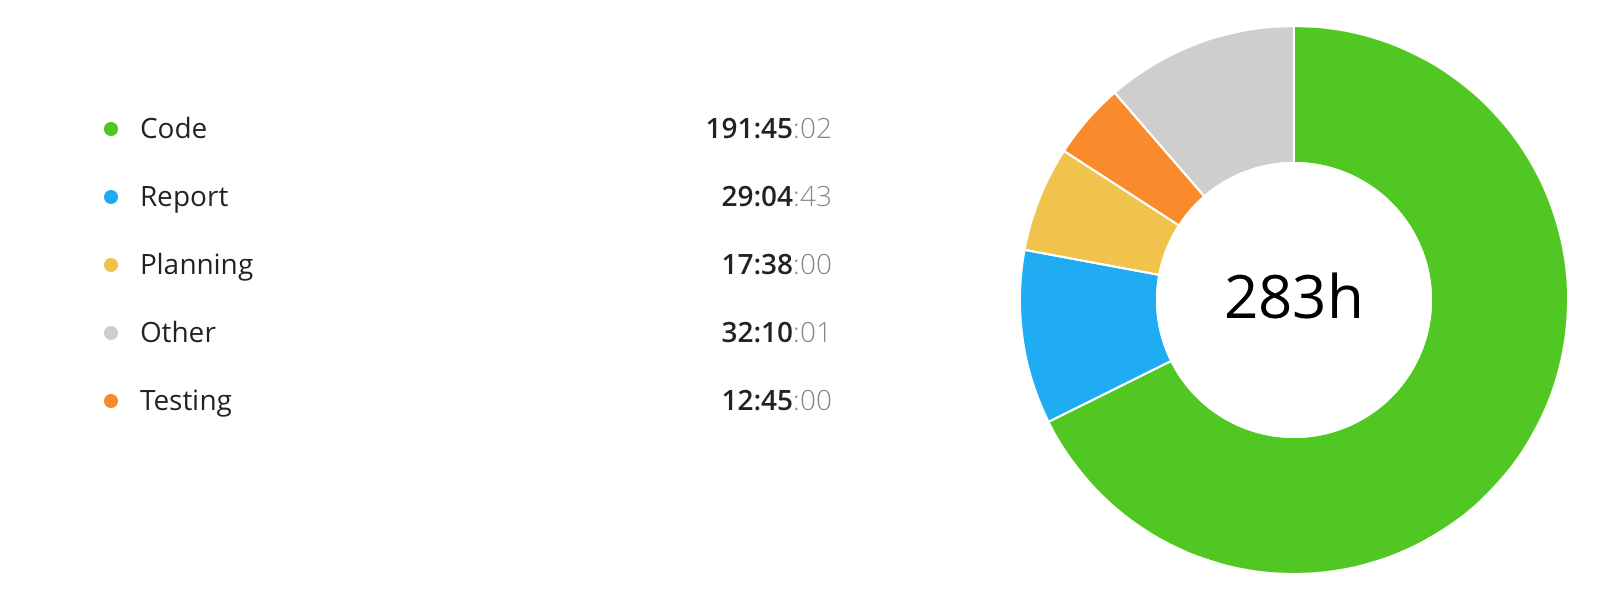
\includegraphics[width=0.8\textwidth]{fig/sprint2-diagram}
\caption{Sprint 2, hours distributed to work tasks}
\end{figure}

\section{Sprint 4}
\label{Sprints-sprint4}

During the sprint planning, the group went through the product backlog once more and prioritized and re-estimated the workload. The group had previously decided that sprint four was the last sprint where the group could implement new features (see section \ref{s:sprints}). The last couple of weeks of the project should be used to clean up code, fix bugs and focus on documentation. 

The group discussed adding a new feature, robots.txt. Robots.txt, is used to inform web robots not to index any images or other static information. The feature was agreed upon, because of its low cost of implementation and its privacy boost. 

The first thing that was finalized in sprint 4, was the easy installation and guide. The rest of the sprint went really well and there were none problems or other issues during the sprint, all features was implemented.

The group conducted a focus-group test with providers and possible system maintainers (see \ref{before_focus_group_with_providers}). Group members Skaugvoll and Norstein, represented and held the test on behalf of the group. The group demonstrated a few possible scenarios and the main concepts. 


\begin{figure}[ht]
\centering
    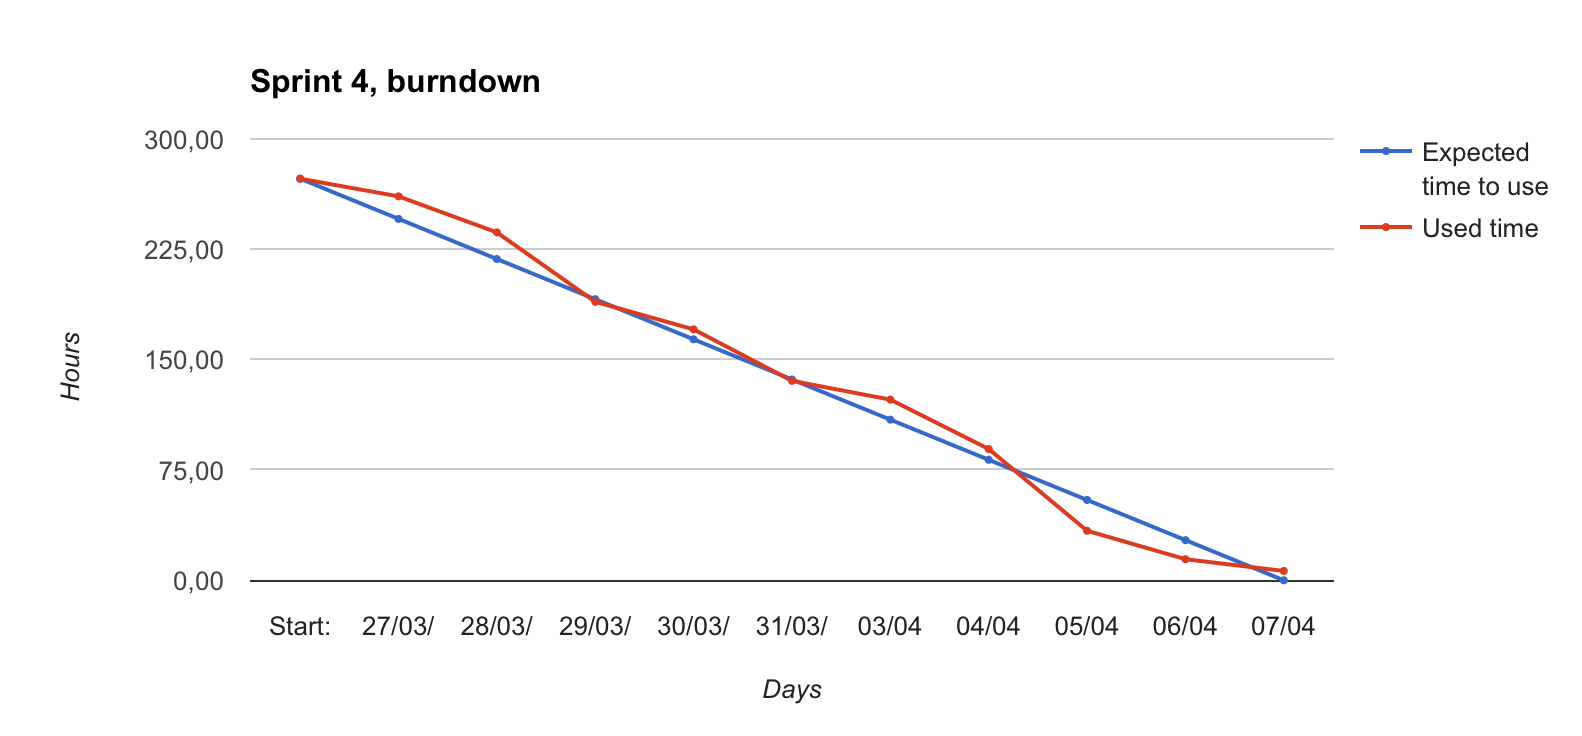
\includegraphics[width=0.8\textwidth]{fig/sprint4}
\caption{Sprint 4, burndown}
\end{figure}

\begin{figure}[ht]
\centering
    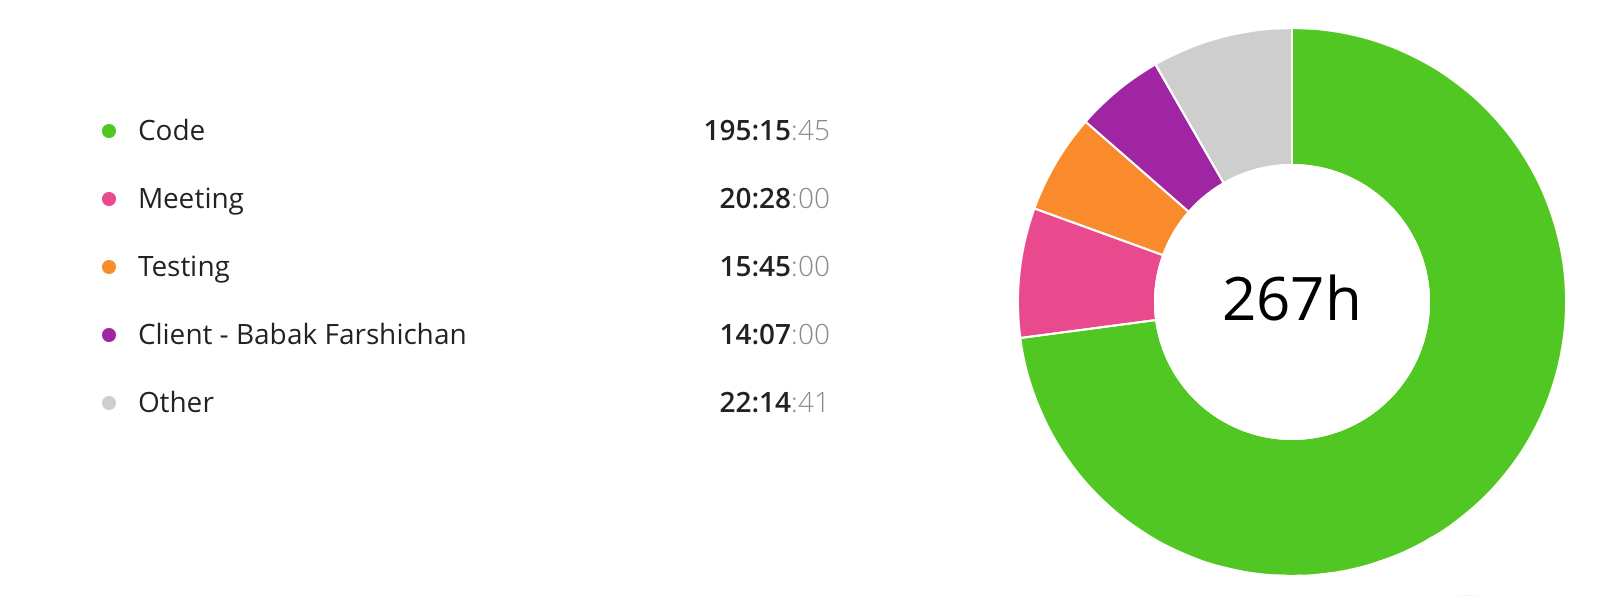
\includegraphics[width=0.8\textwidth]{fig/sprint4-diagram}
\caption{Sprint 4, hours distributed to work tasks}
\end{figure}

\section{Sprint 5}
\label{Sprints-sprint5}

The sprint ended with structuring and cleaning of the code. The information on GitHub was also updated so that the product could be delivered to the customer as complete and documented as possible.

\begin{figure}[ht]
\centering
    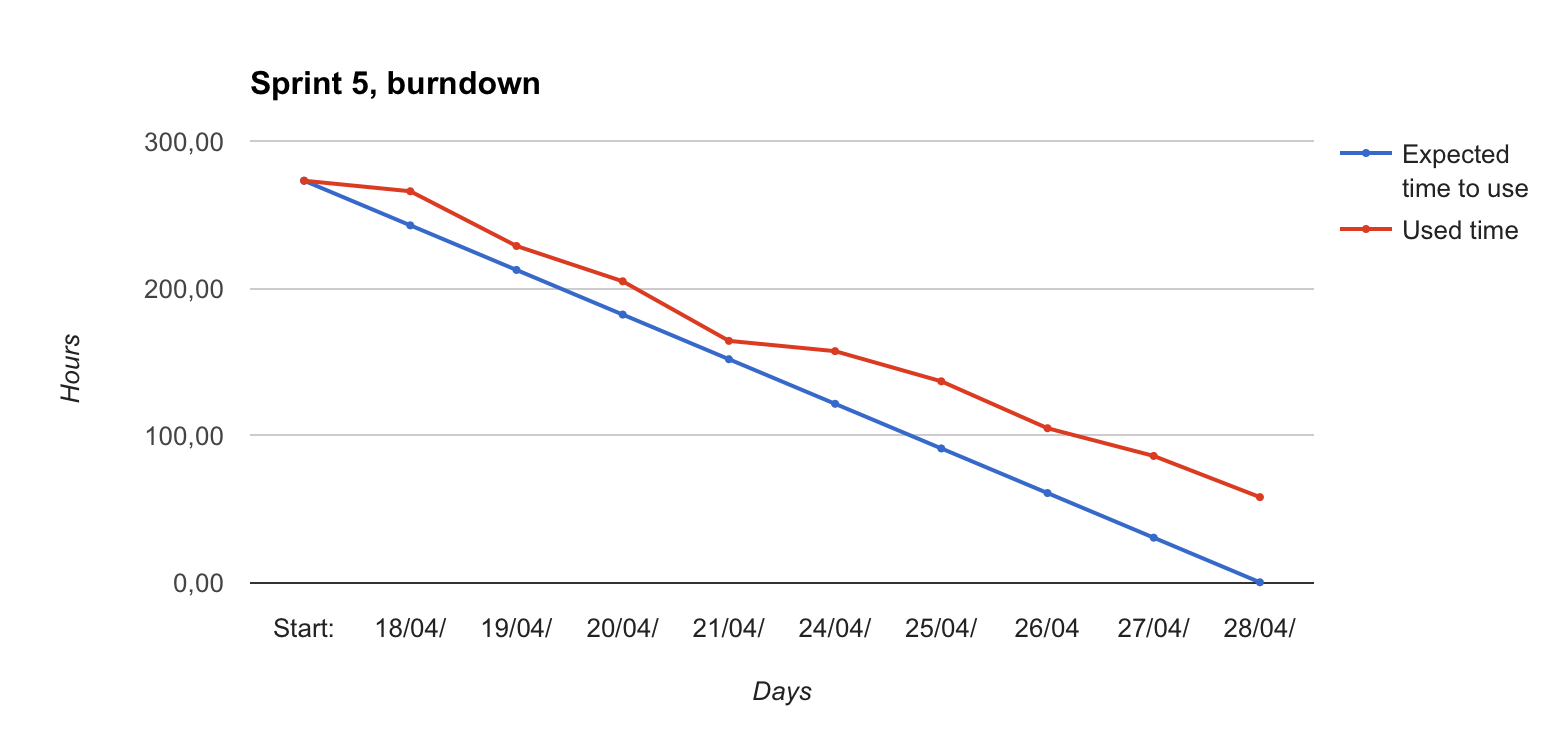
\includegraphics[width=0.8\textwidth]{fig/sprint5}
\caption{Sprint 5, burndown}
\end{figure}

\begin{figure}[ht]
\centering
    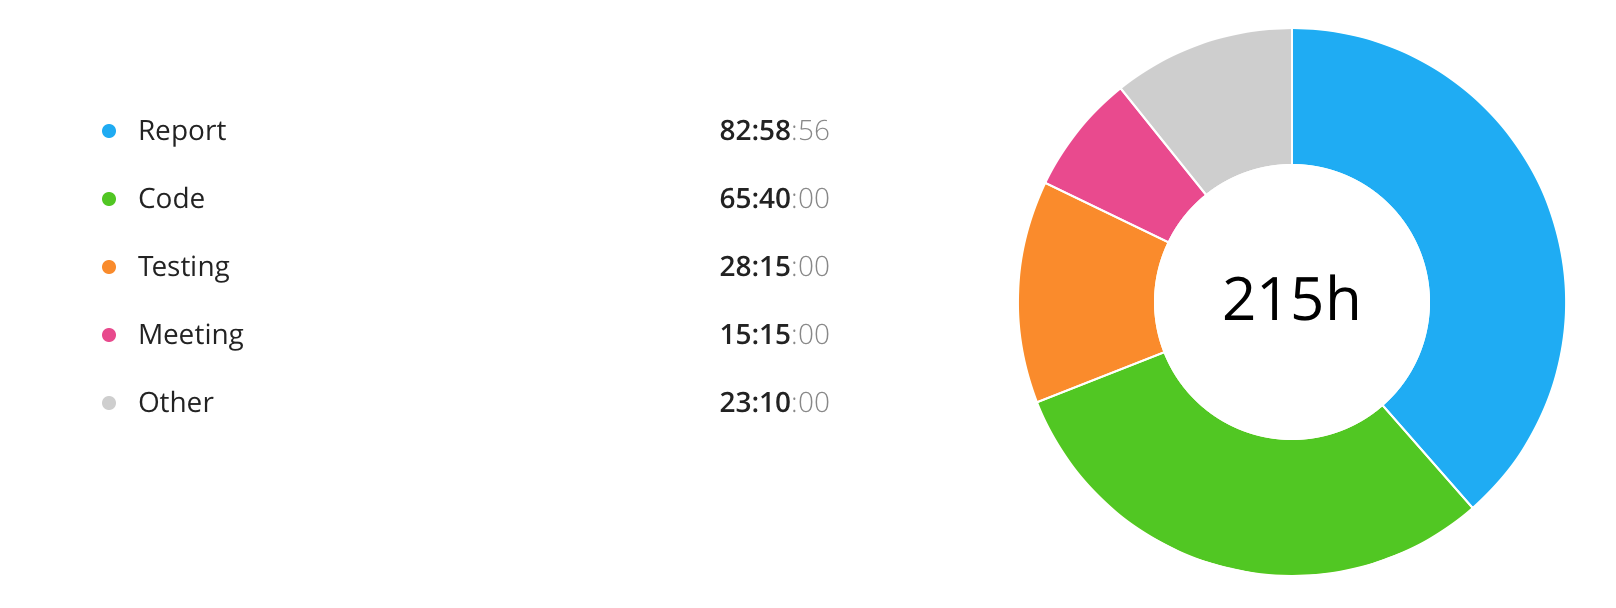
\includegraphics[width=0.8\textwidth]{fig/sprint5-diagram}
\caption{Sprint 5, hours distributed to work tasks}
\end{figure}

\section{Sprint 6}
\label{Sprints-sprint6}

\cleardoublepage